\documentclass[border=6pt]{standalone}
\usepackage{amsmath,amssymb}
\usepackage[dvipsnames]{xcolor}
\usepackage{tikz}
\definecolor{goodpurple}{HTML}{E771DF}
\definecolor{orange(ryb)}{HTML}{FFA500}
\definecolor{dodgerblue}{HTML}{1E90FF}
\colorlet{cz1color}{PineGreen}
\colorlet{cz2color}{LimeGreen}
\begin{document}
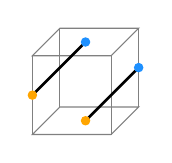
\begin{tikzpicture}[scale = 0.5, baseline={([yshift=-.5ex]current bounding box.center)}]
    \coordinate (A) at (0, 0);
    \coordinate (Azp) at (0, 2);%1.5); % 2 
    \coordinate (Azm) at (0, -1.6); %2
    \coordinate (B) at (0.7, 0.7);
    \coordinate (Bzp) at (0.7, 0.7 + 2);
    \coordinate (C) at (2.7, 0.7);
    \coordinate (Czp) at (2.7, 2.7);
    \coordinate (D) at (2, 0);
    \coordinate (Dzp) at (2, 2);
    \coordinate (E) at (-0.7, -0.7);
    \coordinate (F) at (-2.7, -0.7);
    \coordinate (G) at (-2, 0);
    \coordinate (H) at (-1.3, 0.7);
    \coordinate (I) at (1.3, -0.7);
    %
    \draw[color = gray] (A) -- (B) -- (C) -- (D)--cycle;
    \draw[color = gray] (Azp) -- (Bzp) -- (Czp) -- (Dzp)--cycle;
    \draw[color = gray] (B) -- (Bzp);
    \draw[color = gray] (C) -- (Czp);
    \draw[color = gray] (D) -- (Dzp);
    % \draw[color = gray] (A) -- (E) -- (F) -- (G)--cycle;
    % \draw[color = gray] (A) -- (B) -- (H) -- (G)--cycle;
    % \draw[color = gray] (A) -- (E) -- (I) -- (D)--cycle;
    \draw[color = gray] (A) -- (Azp);    

    
    %gates
    \draw[color = black, line width = 1pt]  (1+0.35,0.35) -- (2+0.7,1+0.7);
    \draw[color = black, line width = 1pt]  (0,1) -- (1+0.35,2+0.35);
    

    % qubits
    % \filldraw[color = goodpurple] (A) circle (3 pt);
    % \filldraw[color = black] (D) circle (3 pt);
    \filldraw[color = orange(ryb)] (0,1) circle (3 pt);
    \filldraw[color = orange(ryb)] (1+0.35,0.35) circle (3 pt);
    \filldraw[color = dodgerblue] (1+0.35,2+0.35) circle (3 pt);
    \filldraw[color = dodgerblue] (2+0.7,1+0.7) circle (3 pt);

    
    % \node at (-0.25, -0.25) {\scriptsize $\mathbf{v}$};
\end{tikzpicture}
\end{document}
